\chapter{Diffraction}

\section{Fraunhofer Diffraction}

\subsection{Single-slit}

\begin{figure}[H]
  \centering
  \begin{subfigure}{.5\textwidth}
    \centering
    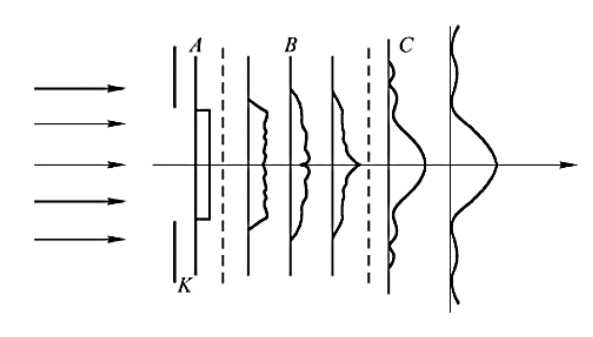
\includegraphics[width=\linewidth]{figures/Fraunhofer-Fresnel-Diffraction}
  \end{subfigure}
  \begin{subfigure}{.45\textwidth}
    \centering
    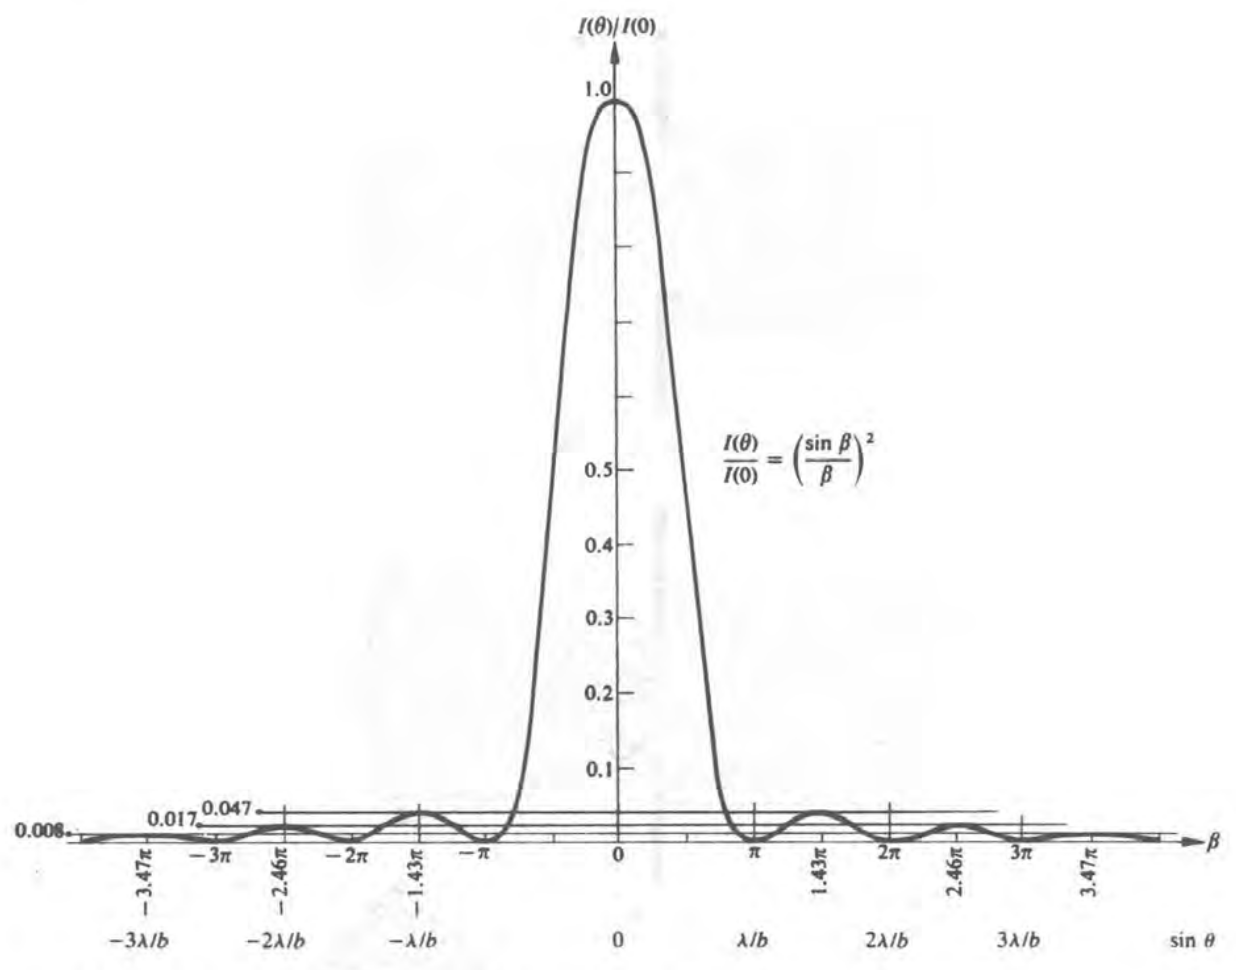
\includegraphics[width=\linewidth]{figures/Fraunhofer-Diffraction-Irradance}
  \end{subfigure}
\end{figure}

White fringes:

\begin{equation*}
  \left\{
    \begin{aligned}
      b \sin \theta &= 0 && \quad\quad \text{(For central fringe)} \\
      \sin \theta &= \pm \dfrac{\left( 2 m + 1 \right)}{2} \cdot \dfrac{\lambda}{b} && \quad\quad m = 1,2,3,\dots
    \end{aligned}
  \right.
  \quad\quad 
  \left\{
    \begin{aligned}
      \Delta \theta_0 &= 2 \cdot \dfrac{\lambda}{b} \\
      \Delta \theta &= \dfrac{\lambda}{b} 
    \end{aligned}
  \right.
\end{equation*}

Dark fringes:

\begin{equation*}
  \begin{aligned}
    \sin \theta = \pm m \cdot \dfrac{\lambda}{b} \quad\quad m = 1,2,3,\dots
  \end{aligned}
\end{equation*}

Irradiance

\begin{equation*}
  \begin{aligned}
    I_p = I_0 \dfrac{\sin^2 u}{u^2}
    \quad\quad
    u = \dfrac{\pi b \sin \theta}{\lambda} 
  \end{aligned}
\end{equation*}

\subsection{Double-slit}

\begin{figure}[H]
  \centering
  \begin{subfigure}{.35\textwidth}
    \centering
    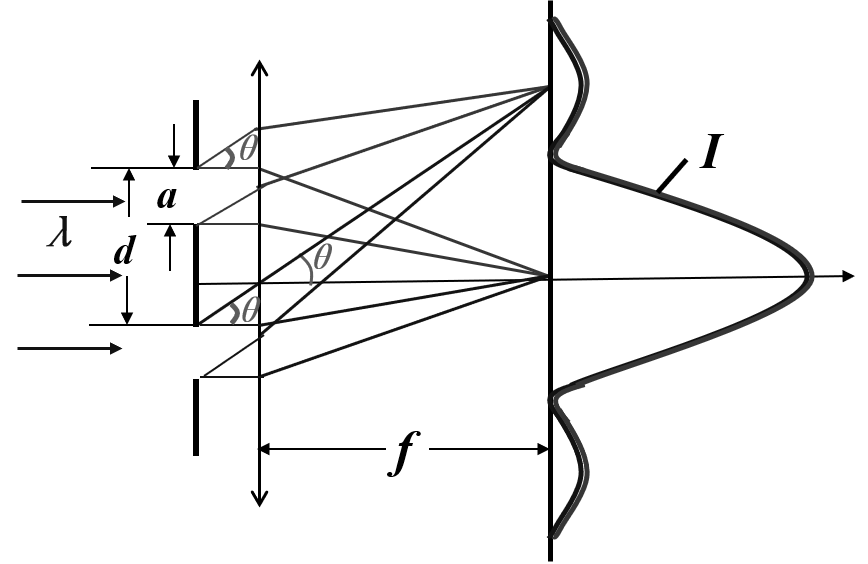
\includegraphics[width=\linewidth]{figures/double-slit-diffraction.png}
  \end{subfigure}
  \begin{subfigure}{.6\textwidth}
    \centering
    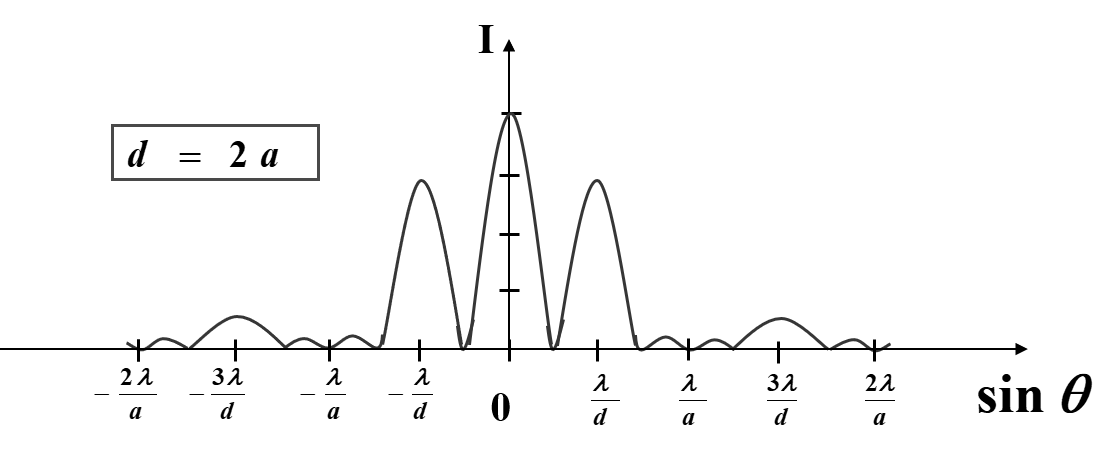
\includegraphics[width=\linewidth]{figures/double-slit-diffraction-irradiance.png}
  \end{subfigure}
\end{figure}

White fringe caused by interference:

\begin{equation*}
  \begin{aligned}
    \sin \theta_I = \dfrac{k \lambda}{d}, k = 0,\pm 1, \pm 2, \dots
  \end{aligned}
\end{equation*}

Dark fringe caused by diffraction:

\begin{equation*}
  \begin{aligned}
    \sin \theta_d = \pm m \cdot \dfrac{\lambda}{a}, m = 1,2,3,\dots 
  \end{aligned}
\end{equation*}

Fringe will cancel when:

\begin{equation*}
  \begin{aligned}
    \dfrac{k \lambda}{d} = m \cdot \dfrac{\lambda}{a} \quad \Rightarrow \quad k = \dfrac{d}{a} m  
  \end{aligned}
\end{equation*}

Irradiance:

\begin{equation*}
  \begin{aligned}
    I = 4 I_0 \dfrac{\sin^2 \left( \dfrac{\pi a \sin \theta}{\lambda} \right)}{\left( \dfrac{\pi a \sin \theta}{\lambda}  \right)^2} \cos^2 \left( \dfrac{\pi d \sin \theta }{\lambda}  \right)
  \end{aligned}
\end{equation*}

\section{Grating}

\begin{figure}[H]
  \centering
  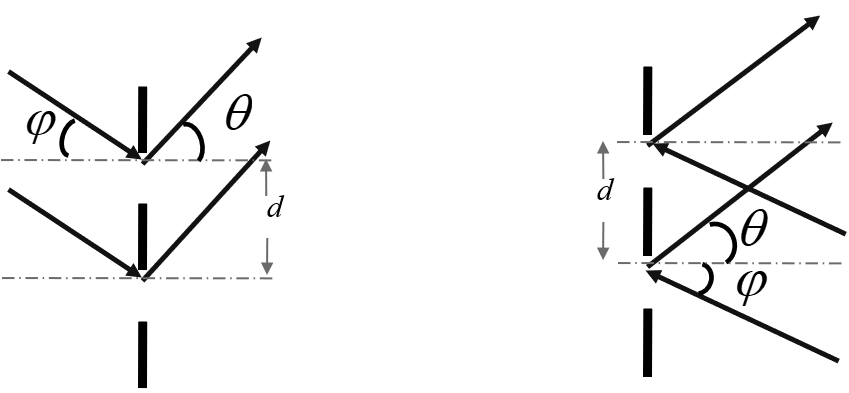
\includegraphics[width=0.5\linewidth]{figures/grating.png}
\end{figure}

Grating equation

\begin{equation*}
  \begin{aligned}
    & d \left( \sin \theta + \sin \phi \right) = m \lambda
    \quad\quad
    \lambda = 0, \pm 1, \pm 2, \dots
    \quad \Rightarrow \quad 
    d \cos \theta \Delta \theta = \Delta \lambda
  \end{aligned}
\end{equation*}

Dispersion:

\begin{equation*}
  \begin{aligned}
    & D_{\theta} = \dfrac{\Delta \theta}{\Delta \lambda} = \dfrac{m}{d \cos \theta}
    \quad\quad 
    D_l = D_{\theta} f = \dfrac{m f}{\cos \theta} 
  \end{aligned}
\end{equation*}

least resolvable difference

\begin{equation*}
  \begin{aligned}
    & \Delta \lambda_{min} = \dfrac{\lambda}{N m}
  \end{aligned}
\end{equation*}

resolving power

\begin{equation*}
  \begin{aligned}
    & R = \dfrac{\lambda}{\Delta \lambda} = mN 
  \end{aligned}
\end{equation*}

free spectrum range

\begin{equation*}
  \begin{aligned}
    & \lambda_{SR} = \dfrac{\lambda}{m} 
  \end{aligned}
\end{equation*}

\section{Blazed Grating}

\begin{minipage}[htbp]{0.6\linewidth}
  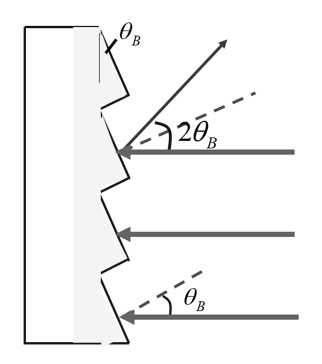
\includegraphics[width=0.4\linewidth]{figures/blazed-grating.png}
  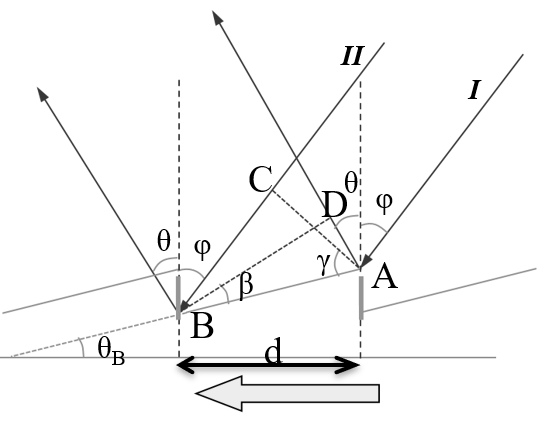
\includegraphics[width=0.6\linewidth]{figures/blazed-grating-1.png}
\end{minipage}
\begin{minipage}[htbp]{0.4\linewidth}
  \begin{equation*}
    \begin{aligned}
      & \sin \phi + \sin \left( 2 \theta_B - \phi \right) = \dfrac{m\lambda}{d} \\
      & I = I_0 \cdot \dfrac{\sin^2 u}{u^2} \cdot \dfrac{\sin^2 N \nu}{\sin^2 \nu} \\
      & \nu = \dfrac{\pi d}{\lambda} \left( \sin \phi + \sin \theta \right) \\
      & u = \dfrac{\pi d}{\lambda \cos \theta_B} \left[ \sin \left( \theta - \theta_B \right) + \left( \sin \left( \phi - \theta_B \right) \right) \right] 
    \end{aligned}
  \end{equation*}
\end{minipage}

\section{Fresnel Diffraction}

\begin{figure}[H]
  \centering
  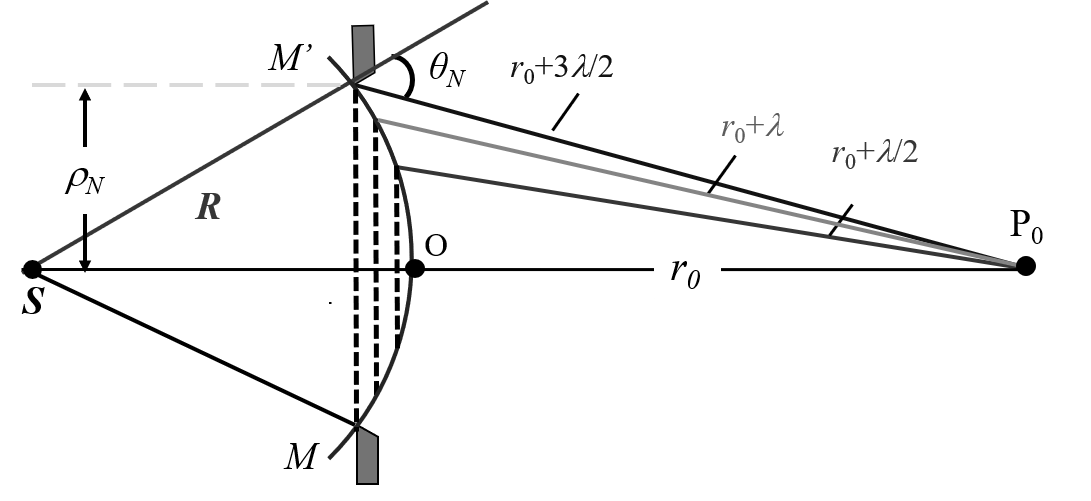
\includegraphics[width=0.7\linewidth]{figures/fresnel.png}
\end{figure}

\begin{equation*}
  N = \dfrac{\rho_N^2}{\lambda R} \left( 1 + \dfrac{R}{r_0}  \right) =
  \left\{
  \begin{aligned}
    & \dfrac{\rho_N^2}{\lambda r_0} && R \rightarrow \infty
    \quad \Rightarrow \quad
    f = \dfrac{\rho_N^2}{\lambda N} \\ 
    \\
    & \dfrac{\rho_N^2}{\lambda R} && r_0 \rightarrow \infty \\
    \\
    & 0 && R \rightarrow \infty \text{ and } r_0 \rightarrow \infty 
  \end{aligned}
  \right.
\end{equation*}




%%% Local Variables:
%%% mode: latex
%%% TeX-master: "Optics"
%%% End:
